\section{Counterfactual Explanations}
We propose a new explanation modality -- counterfactual explanations.
Using a slight modification to \gcam{}, we can obtain explanations
that highlight support for regions that would make the network change its prediction.
As a consequence, removing concepts occurring in those regions would make the
model more confident about its prediction.

Specifically, we negate the gradient of $y^c$ (score for class $c$) with respect to feature maps $A$ of a convolutional layer.
Thus the importance weights $\alpha{}_{k}^{c}$ now become
\begin{ceqn}
\begin{equation} \label{eq:alpha_neg}
    \alpha{}_{k}^c =
    \overbrace{
        \frac{1}{Z}\sum_{i}\sum_{j}
    }^{\text{global average pooling}}
    \hspace{-17pt}
    \underbrace{
        \vphantom{\sum_{i}\sum_{j}} -\frac{\partial y^c}{\partial A_{ij}^{k}}
    }_{\text{Negative gradients}}
\end{equation}
\end{ceqn}
As in \eqref{eq:gcam}, we take a weighted sum of the forward activation maps, $A$, with weights $\alpha{}_{k}^c$, and follow it by a ReLU to obtain counterfactual explanations as shown in \reffig{fig:negexp}.

\begin{figure}[ht!]
    \centering \begin{subfigure}[t]{0.158\textwidth} \centering
        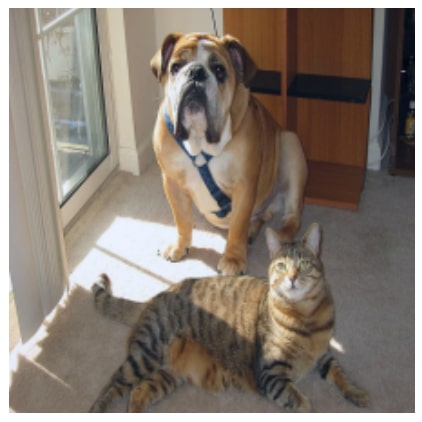
\includegraphics[width=\textwidth]{figures/teaser/original.jpg}
        \caption{\scriptsize{Original Image}}
	\end{subfigure}
	\begin{subfigure}[t]{0.158\textwidth}
        \centering
        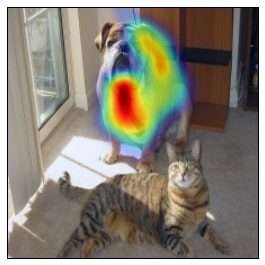
\includegraphics[width=\textwidth]{figures/cat_neg_exp.jpg}
        \caption{\scriptsize{Cat Counterfactual exp}}
		\label{fig:neg_exp_cat}
	\end{subfigure}
    \centering
	\begin{subfigure}[t]{0.158\textwidth}
        \centering
        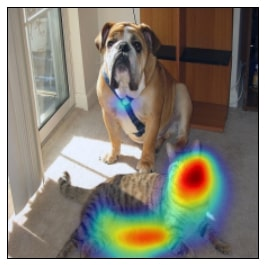
\includegraphics[width=\textwidth]{figures/dog_neg_exp.jpg}
        \caption{\ijcv{\scriptsize{\hspace{-1pt}Dog Counterfactual exp}}}%
		\label{fig:neg_exp_dog}
	\end{subfigure}
    \vspace{10pt}
    \caption{Counterfactual Explanations with \gcam{}}
    \label{fig:negexp}
\end{figure}
